%! Suppress = TooLargeSection
%%%%%%%%%%%%%%%%%%%%%%%%%%%%%%%%%%%%%%%%%%
%                                        %
% Szablon pracy dyplomowej magisterskiej %
%                                        %
%%%%%%%%%%%%%%%%%%%%%%%%%%%%%%%%%%%%%%%%%%



\documentclass[a4paper,twoside,12pt]{book}
\usepackage[utf8]{inputenc}
\usepackage[T1]{fontenc}
\usepackage{amsmath,amsfonts,amssymb,amsthm}
\usepackage[british,polish]{babel}
\usepackage{indentfirst}
\usepackage{lmodern}
\usepackage{graphicx}
\usepackage{hyperref}
\usepackage{booktabs}
\usepackage{tikz}
\usepackage{pgfplots}
\usepackage{mathtools}
\usepackage[page]{appendix} % toc,
\renewcommand{\appendixtocname}{Dodatki}
\renewcommand{\appendixpagename}{Dodatki}
\renewcommand{\appendixname}{Dodatek}

\usepackage{setspace}
\onehalfspacing


\frenchspacing

\usepackage{listings}
\lstset{
language={},
basicstyle=\ttfamily,
keywordstyle=\lst@ifdisplaystyle\color{blue}\fi,
commentstyle=\color{gray}
}

%%%%%%%%%

%%%% LIST GENERATOR %%%%%%%%%

%\usepackage{tikz}
%\usepackage{manfnt}   % dangerous sign
\usepackage{color}
\definecolor{brickred}      {cmyk}{0 , 0.89, 0.94, 0.28}

\makeatletter \newcommand \kslistofremarks{\section*{Uwagi} \@starttoc{rks}}
\newcommand\l@uwagas[2]
{\par\noindent \textbf{#2:} %\parbox{10cm}
{#1}\par} \makeatother


\newcommand{\ksremark}[1]{%
{%\marginpar{\textdbend}
{\color{brickred}{[#1]}}}%
\addcontentsline{rks}{uwagas}{\protect{#1}}%
}

\newcommand{\comma}{\ksremark{przecinek}}
\newcommand{\nocomma}{\ksremark{bez przecinka}}
\newcommand{\styl}{\ksremark{styl}}
\newcommand{\ortografia}{\ksremark{ortografia}}
\newcommand{\fleksja}{\ksremark{fleksja}}
\newcommand{\pauza}{\ksremark{pauza `--', nie dywiz `-'}}
\newcommand{\kolokwializm}{\ksremark{kolokwializm}}

%%%%%%%%%%%%%% END OF GENERATOR %%%%%%%%%%%

%%%%%%%%%%%% ZYWA PAGINA %%%%%%%%%%%%%%%
% brak kapitalizacji zywej paginy
\usepackage{fancyhdr}
\pagestyle{fancy}
\fancyhf{}
\fancyhead[LO]{\nouppercase{\it\rightmark}}
\fancyhead[RE]{\nouppercase{\it\leftmark}}
\fancyhead[LE,RO]{\it\thepage}


\fancypagestyle{tylkoNumeryStron}{%
\fancyhf{}
\fancyhead[LE,RO]{\it\thepage}
}

\fancypagestyle{NumeryStronNazwyRozdzialow}{%
\fancyhf{}
\fancyhead[LO]{\nouppercase{\it\rightmark}}
\fancyhead[RE]{\nouppercase{\it\leftmark}}
\fancyhead[LE,RO]{\it\thepage}
}


%%%%%%%%%%%%% OBCE WTRETY
\newcommand{\obcy}[1]{\emph{#1}}
\newcommand{\ang}[1]{{\selectlanguage{british}\obcy{#1}}}
%%%%%%%%%%%%%%%%%%%%%%%%%%%%%

% polskie oznaczenia funkcji matematycznych
\renewcommand{\tan}{\operatorname {tg}}
\renewcommand{\log}{\operatorname {lg}}

% jeszcze jakies drobiazgi

\newcounter{stronyPozaNumeracja}

\newcommand{\hcancel}[1]{%
\tikz[baseline=(tocancel.base)]{
\node[inner sep=0pt,outer sep=0pt] (tocancel) {#1};
\draw[red] (tocancel.south west) -- (tocancel.north east);
}%
}%

\newcommand{\miesiac}{%
\ifcase\the\month
\or styczeń% 1
\or luty% 2
\or marzec% 3
\or kwiecień% 4
\or maj% 5
\or czerwiec% 6
\or lipiec% 7
\or sierpień% 8
\or wrzesień% 9
\or październik% 10
\or listopad% 11
\or grudzień% 12
\fi}


%%%%%%%%%%%%%%%%%%%%%%%%%%%%%%%%%%%%%%%%%%%%%%
%%%%%%%%%%%%%%%%%%%%%%%%%%%%%%%%%%%%%%%%%%%%%%
%%%%%%%%%%%%%%%%%%%%%%%%%%%%%%%%%%%%%%%%%%%%%%
%%%%%%%%%%%%%%%%%%%%%%%%%%%%%%%%%%%%%%%%%%%%%%
%%%%%%%%%%%%%%%%%%%%%%%%%%%%%%%%%%%%%%%%%%%%%%
%%%%%%%%%%%%%%%%%%%%%%%%%%%%%%%%%%%%%%%%%%%%%%
%%%%%%%%%%%%%%%%%%%%%%%%%%%%%%%%%%%%%%%%%%%%%%
%%%%%%%%%%%%%%%%%%%%%%%%%%%%%%%%%%%%%%%%%%%%%%


\newcommand{\autor}{Mateusz Trzeciak}
\newcommand{\promotor}{dr hab.
inż.
Karolina Nurzyńska}
\newcommand{\tytul}{Określenie wieku twarzy na podstawie tekstury}


\begin{document}
    %\kslistofremarks

    %%%%%%%%%%%%%%%%%%  STRONA TYTULOWA %%%%%%%%%%%%%%%%%%%
    \pagestyle{empty}
    \sffamily

    \noindent

    \begin{center}
        \large
        Politechnika Śląska\\
        Wydział Automatyki, Elektroniki i~Informatyki \\
        kierunek: informatyka
    \end{center}

    \vfill\vfill
    \begin{center}
        \large
        \autor
    \end{center}

    \vfill
    \begin{center}
        \LARGE\bfseries \tytul
    \end{center}

    \vfill
    \begin{center}
        \large
        praca dyplomowa magisterska
    \end{center}

    \vfill\vfill\vfill
    \begin{center}
        \large
        \begin{tabular}{ll}
            promotor: & \promotor \\
            % konsultant: & \konsultant \\ % jezeli nie ma, zakomentowac
        \end{tabular}

    \end{center}

    \vfill
    \begin{center}
        \large
        Gliwice,  \miesiac\ \the\year
    \end{center}

    \cleardoublepage


    \rmfamily
    \normalfont

    %%%%%%%%%%%%%%%%%%%%% oswiadczenie o udostępnianiu pracy dyplomowej %%%%%%%%%%%%%%%%%%%
    \cleardoublepage

    \begin{flushright}
        załącznik nr 2 do zarz.
        nr 97/08/09
    \end{flushright}

    \vfill

    \begin{center}
        \Large\bfseries Oświadczenie
    \end{center}

    \vfill

    Wyrażam zgodę / Nie wyrażam zgody* na udostępnienie mojej pracy dyplomowej / rozprawy doktorskiej*.

    \vfill

    Gliwice, dnia \today

    \vfill

    \rule{0.5\textwidth}{0cm}\dotfill

    \rule{0.5\textwidth}{0cm}
    \begin{minipage}{0.45\textwidth}
    {\begin{center}
         (podpis)
    \end{center}}
    \end{minipage}

    \vfill

    \rule{0.5\textwidth}{0cm}\dotfill

    \rule{0.5\textwidth}{0cm}
    \begin{minipage}{0.45\textwidth}
    {\begin{center}
         \rule{0mm}{5mm}(poświadczenie wiarygodności podpisu przez Dziekanat)
    \end{center}}
    \end{minipage}


    \vfill

    * podkreślić właściwe




    %%%%%%%%%%%%%%%%%%%%% oswiadczenie promotora o spełnieniu wymagań formalnych %%%%%%%%%%%%%%%%%%%
    \cleardoublepage

    \rule{1cm}{0cm}

    \vfill

    \begin{center}
        \Large\bfseries Oświadczenie promotora
    \end{center}

    \vfill

    Oświadczam, że praca „\tytul” spełnia wymagania formalne pracy dyplomowej magisterskiej.

    \vfill



    \vfill

    Gliwice, dnia \today

    \rule{0.5\textwidth}{0cm}\dotfill

    \rule{0.5\textwidth}{0cm}
    \begin{minipage}{0.45\textwidth}
    {\begin{center}
         (podpis promotora)
    \end{center}}
    \end{minipage}

    \vfill

    %\rule{0.5\textwidth}{0cm}\dotfill
    %
    %\rule{0.5\textwidth}{0cm}
    %\begin{minipage}{0.45\textwidth}
    %{\begin{center}\rule{0mm}{5mm}(poświadczenie wiarygodności podpisu przez Dziekanat)\end{center}}
    %\end{minipage}
    %
    %
    %\vfill



    \cleardoublepage


    %%%%%%%%%%%%%%%%%% SPIS TRESCI %%%%%%%%%%%%%%%%%%%%%%
    \pagenumbering{Roman}
    \pagestyle{tylkoNumeryStron}
    \tableofcontents

    %%%%%%%%%%%%%%%%%%%%%%%%%%%%%%%%%%%%%%%%%%%%%%%%%%%%%
    \setcounter{stronyPozaNumeracja}{\value{page}}
    \mainmatter
    \pagestyle{NumeryStronNazwyRozdzialow}

    %%%%%%%%%%%%%% wlasciwa tresc pracy %%%%%%%%%%%%%%%%%

    \chapter{Wstęp}\label{ch:wstęp}

    %\begin{itemize}
    %\item wprowadzenie w problem/zagadnienie
    %\item osadzenie problemu w dziedzinie
    %\item cel pracy
    %\item zakres pracy
    %\item zwięzła charakterystyka rozdziałów
    %\item jednoznaczne określenie wkładu autora
    %\end{itemize}
    Wiek jest cechą, którą niełatwo człowiekowi odczytać z czyjejś twarzy.
    Dla komputera rozpoznawanie wieku jest
    trudniejsze niż dla człowieka.
    Dlatego do wyznaczania wieku z pomocą programu komputerowego należy podchodzić z dystansem.
    Mimo trudności programiści
    i naukowcy udoskonalają algorytmy,
    tak aby ocena wieku danej osoby była coraz dokładniejsza.

    Istnieje wiele sposobów wyznaczania wieku.
    Większość metod skupia się na analizie tekstury twarzy.
    Idąc dalej - z obrazu danej osoby lub jego części, np tułowia,
    musi zostać wykryta twarz.
    Wykrycie twarzy na teksturze jest możliwe dzięki algorytmom rozpoznawaniu obrazu.
    Rozpoznawanie obrazu jest stosowane w wizji komputerowej i polega na wyodrębnieniu z obrazu jakichś szczegółów.
    Mogą
    to być osoby, pojazdy, przedmioty itp. (Rys.~\ref{fig.rozpoznawanieObiektow})

    \begin{figure}
        \centering
        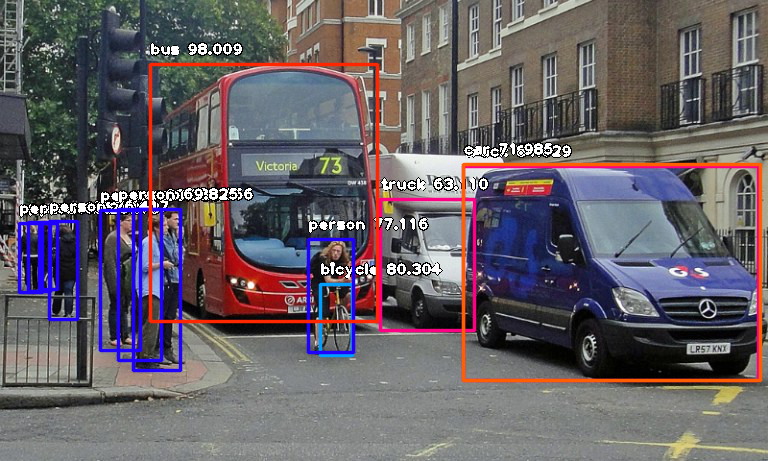
\includegraphics[width=11cm]{Obrazy/rozpoznawanieObiektow.jpeg}
        \caption{Przykład rozpoznawania obiektów na zdjęciu ulicy.~\cite{rozpoznawanieObiektow}}
        \label{fig.rozpoznawanieObiektow}
    \end{figure}

    Można znaleźć wiele witryn internetowych, które udostępniają interfejsy programistyczne umożliwiające zaimplementowanie
    rozpoznawania wieku z obrazu.
    Istnieją algorytmy przetwarzania obrazu, które oprócz wieku wyznaczają z pewnym prawdopodobieństwem płeć danej osoby.
    Oprócz płci mogą one także wyznaczyć mine oraz czy dana osoba nosi okulary.

    Z weryfikacją wieku danej osoby można się spotkać przed wejściem do niektórych miejsc, tj.
    klub nocny.
    Większość osób
    musi okazać ważny dowód osobisty,
    co generuje duże kolejki do wejścia.
    Aplikacje analizujące wiek na podstawie obrazu twarzy z kamery przed wejściem
    do takich miejsc znacząco usprawniłyby weryfikację wieku.
    Rozpoznawanie wieku może być wykorzystywane przy analizie średniego wieku ludzi w jakimś miejscu np.
    podczas demonstracji.

    Wiele gier posiada treści nieodpowiednie dla młodszych użytkowników.
    Możliwe jest stosowanie technologii wykrywania
    wieku użytkownika przed udostępnieniem mu treści, która wymaga odpowiedniego wieku.

    Można znaleźć o wiele więcej potencjalnych zastosowań przetwarzania obrazu oraz rozpoznawania wieku na podstawie
    tekstury (obrazu) twarzy.
    Z biegiem lat z pewnością będzie można zauważyć dalszy rozwój tej dziedziny, która
    opiera się w głównej mierze na sztucznej inteligencji~\cite{computerVision}.
    %275 wyrazow

    %    \section{Cel i zakres pracy}
    %    Celem pracy magisterskiej jest stworzenie prostego programu do rozpoznawania wieku na podstawie tekstury twarzy.
    %
    %    Zakres pracy obejmuje:
    %    \begin{itemize}
    %        \item Wybór bazowej metody wyznaczania wieku
    %        \item Stworzenie kilku modyfikacji bazowej metody
    %        \item Opis algorytmów każdej z metod wyznaczania wieku
    %        \item Porównanie wszystkich metod i wybór najlepszej
    %    \end{itemize}
    %
    %    \chapter{Przegląd metod wyznaczania wieku}
    %    \section{Metoda a}
    %    \section{Metoda b}
    %    \section{Metoda wrinkle feature}

    \chapter{Metoda bazowa - wrinkle feature}\label{ch:metoda-bazowa---wrinkle-feature}

    Istnieje wiele metod wyznaczania wieku z obrazu twarzy.
    W literaturze spotkano rozwiązania, w których wyznaczany
    jest konkretny
    wiek osoby przez algorytm lub przedział wiekowy.
    Jedna z pierwszych metod szacowania wieku opierała się na wyznaczaniu proporcji twarzy, a następnie na detekcji i
    interpretacji zmarszczek.
    Była ona w stanie ze stu procentową poprawnością wyznaczyć czy dana osoba jest osobą
    dorosłą lub
    dzieckiem~\cite{kwonLobo}.

    W kolejnych latach algorytmy i techniki szacowania wieku były udoskonalane.
    Badano wpływ starzenia się osób na
    wygląd skóry.
    Oprócz naturalnych zmian skóry pod wpływem starzenia się skóry należało uwzględnić także inne
    czynniki.
    Takimi czynnikami są min.
    płeć, poziom stresu, ekspozycja na działanie środowiska zewnętrznego.
    Powyższe metody zastosowano w pracy ,,Toward automatic simulation
    of aging effects on face images'' autorstwa A. Lanitis, Ch. J. Taylor oraz T. F. Cootes~\cite{lanitisTaylor}.
    Należy dodać, że w powyższej pracy stosowano trenowanie zbioru zdjęć.
    Trenowanie polega na wykryciu relacji pewnych cech twarzy do wieku osób.

    W kolejnych latach pojawiło się podejście porównywania cech twarzy tej samej osoby w różnym wieku.
    Różnice w powyższych cechach posłużyły do zbudowania statystyki zmian cech twarzy wraz ze starzeniem się.
    Powyższe podejście zostało zaprezentowane w pracy ,,Face verification across age progression''
    autorstwa N. Ramanathan oraz R. Chellappa~\cite{ramanthanChelappa}.

    Rozwinięciem tego pomysłu była praca ,,Automatic age estimation based
    on facial aging patterns'' autorstwa X. Geng, Z. Zhou i K. Smith-Miles~\cite{gengZhou}.
    W tej pracy porównywano sekwencje wielu zdjęć twarzy jednej osoby.
    Zdjęcia przestawiały twarz w różnym wieku.
    Powyższe badania pozwoliły na zbudowanie wzorca starzenia się twarzy.

    Praca ,,A new algorithm for age recognition
    from facial images'' autorstwa M.M. \ Dehshibi oraz A. Bastanfard~\cite{dehshibiBastard} przy szacowaniu wieku
    analizuje proporcje twarzy oraz ilość zmarszczek.

    Praca ,,Age Estimation from Face Images: Challenging
    Problem for Audience Measurement Systems'' autorstwa
    Vladimira Khryashcheva, Alexandra Ganina, Olgi Stepanovej oraz
    Antona Lebedeva podsumowała techniki szacowania wieku~\cite{khryashchevGanin}.
    Z podsumowania wynikło, że najczęściej stosuje się do wyodrębniania cech z twarzy BIF,
    czyli biologically inspired features.
    Powyższa metoda została zaprezentowana w książce ,,Human Age Estimation Using Bio-inspired Features''
    autorstwa Guodong Guo i in.
    Mniej popularne metody analizujące cechy twarzy to filtry Gabora oraz LBP- local binary patterns.


    Metoda bazowa została opisana w artykule ,,Age Estimation from Face Image using Wrinkle Features''
    ~\cite{wrinkleFeatures}.
    Wykrywanie wieku dzieli się na kilka faz.
    Na początku należy wykryć twarz.
    Zastosowany algorytm wykrywania został
    opisany w sekcji \ref{sec:metodaWykrywaniaTwarzy}
    Następnie należy wyznaczyć strefy zmarszczkowe na twarzy.
    W artykule~\cite{wrinkleFeatures} udowodniono,
    że istnieje kilka konkretnych stref, w których następuje znacząca zmiana ilości zmarszczek wraz z wiekiem.
    Powyższe strefy zostały wymienione w sekcji \ref{sec:wyznaczanieStref}.
    Sekcja \ref{sec:wykrywanieZmarszczek} przedstawia technikę wykrywania zmarszczek znajdujących się w strefach.
    Wykryte zmarszczki
    pozwalają na obliczenie wrinkle feature dla danej twarzy, zgodnie z opisem w sekcji~\ref{sec:wyliczanieWrinkleFeature}.
    W tym miejscu kończy się faza wyznaczania wrinkle feature dla danej osoby (Rysunek \ref{fig.faza1Algorytmu}).
    Kolejna faza
    jest potrzebna do
    znalezienia relacji pomiędzy wrinkle feature a wiekiem.
    Do tego celu należy zastosować algorytm trenujący, który
    został opisany w sekcji \ref{sec:algorytmTrenowania}.
    Wynikiem algorytmu trenującego jest zbiór danych, który
    należy pogrupować, tak jak to opisano w sekcji \ref{sec:grupowanieDanych}.
    Ostatnią fazą algorytmu jest wykrywanie wieku
    na podstawie wyników działania FCM - sekcja \ref{sec:wyznaczanieWieku} (Rysunek \ref{fig.faza2Algorytmu}).

    \begin{figure}[h]
        \centering
        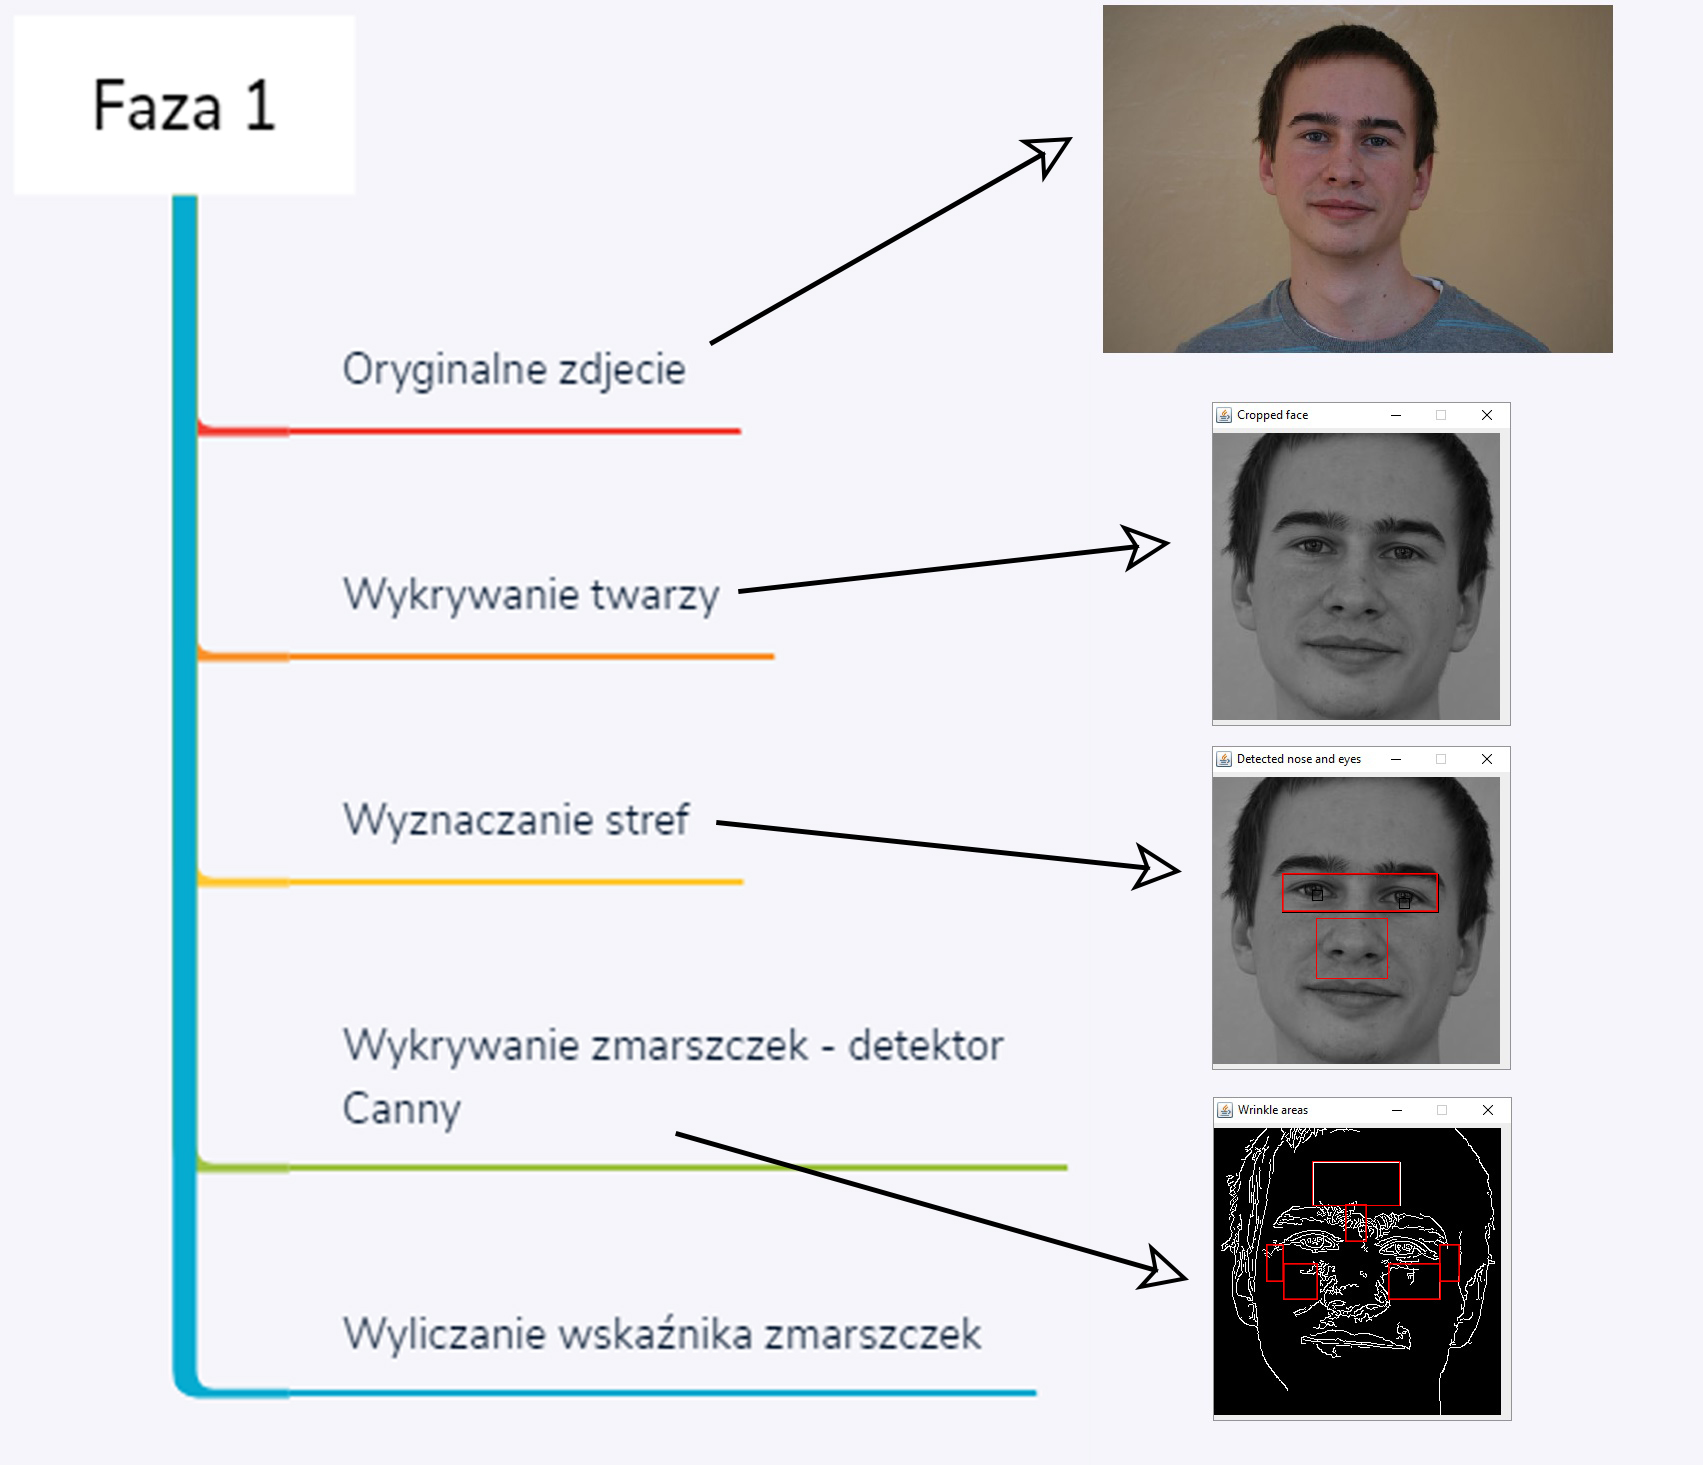
\includegraphics[width=8cm]{Obrazy/Faza1.jpg}
        \caption{Faza 1 algorytmu}
        \label{fig.faza1Algorytmu}
    \end{figure}

    \begin{figure}[h]
        \centering
        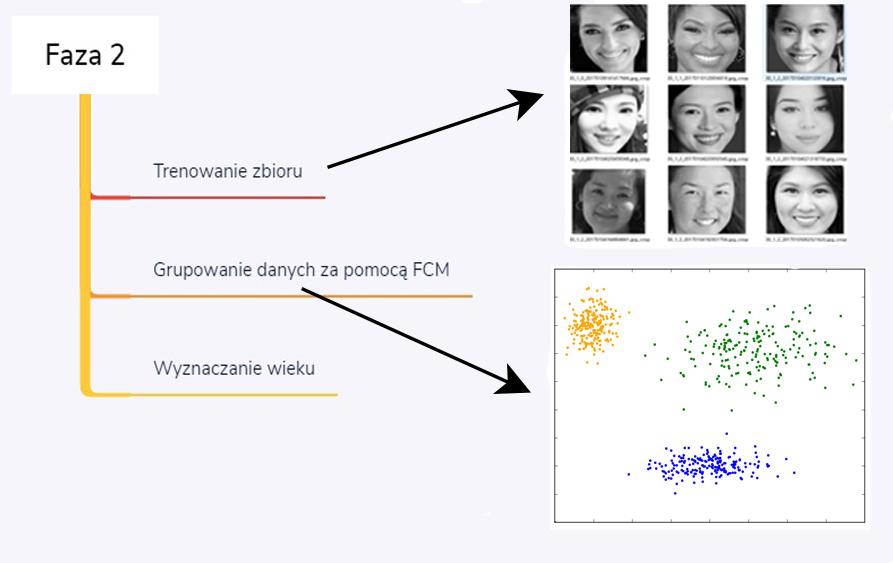
\includegraphics[width=8cm]{Obrazy/Faza2.jpg}
        \caption{Faza 2 algorytmu}
        \label{fig.faza2Algorytmu}
    \end{figure}

    \section{Metoda wykrywania twarzy}\label{sec:metodaWykrywaniaTwarzy}
    W literaturze można odnaleźć wiele metod wykrywania twarzy.
    Istnieje kilka podejść aby skutecznie wykrywać twarz na danym obrazie~\cite{mehdiRizvi}:
    %       https://www.researchgate.net/publication/257338580_A_Review_on_Face_Detection_Methods
    %     Knowledge-based methods: These rule-based methods encode human knowledge
    %    of what constitutes a typical face. Usually, the rules capture the relationships
    %    between facial features. These methods are designed mainly for face localization.
    %     Feature invariant approaches: These algorithms aim to find structural features that
    %    exist even when the pose, viewpoint, or lighting conditions vary, and then use these
    %    to locate faces. These methods are designed mainly for face localization.
    %     Template matching methods: Several standard patterns of a face are stored to
    %    describe the face as a whole or the facial features separately. The correlations
    %    between an input image and the stored patterns are computed for detection. These
    %    methods have been used for both face localization and detection.
    %     Appearance-based methods: In contrast to template matching, the models (or
    %    templates) are learned from a set of training images which should capture the
    %    representative variability of facial appearance. These learned models are then used
    %    for detection. These methods are designed mainly for face detection.

    \begin{itemize}
        \item metoda oparta na nauce
        \item metoda niezmienności cech
        \item metoda dopasowania szablonu twarzy
        \item metoda bazująca na wyglądzie
    \end{itemize}
    Metoda oparta na nauce kieruje się wiedzą na temat wyglądu twarzy, a
    bardziej precyzyjnie chodzi o charakterystyczne cechy,
    dzięki którym na zdjęciu można wyodrębnić obszar twarzy.
    Mowa tutaj o cechach takich jak kształt twarzy, kolor, miejsca o różnej jasności czy specyficzne krawędzie tworzone np przez
    usta.

    W metodzie niezmienności cech wyszukuje się takie strukturalne cechy twarzy, które są widoczne w każdych warunkach
    oświetleniowych.
    Ponadto te cechy są widoczne bez względu na punkt widzenia, nawet jeśli twarz jest widoczna
    z profilu czy przechylona pod kątem.

    Z kolei metoda dopasowania szablonu twarzy wykorzystuje kilka standardowych wzorów opisujących twarz.
    Na wejściu algorytmu obraz jest porównywany z tymi wzorami, a
    na wyjściu dostajemy informację, w jakim stopniu obraz jest dopasowany do szablonu twarzy.

    Ideą metody bazującej na wyglądzie jest trenowanie dużego zbioru obrazów twarzy, tak aby wychwycić zmienność cech
    twarzy.
    Tak wytrenowany model jest później wykorzystywany do wykrywania twarzy.


    Ponadto w procesie ekstrakcji twarzy z obrazu istnieje wiele problemów~\cite{mehdiRizvi}.
    %       https://www.researchgate.net/publication/257338580_A_Review_on_Face_Detection_Methods
    %    Pose: The images of a face vary due to the relative camera-face pose (frontal, 45
    %    degree, profile, upside down), and some facial features such as an eye or the nose
    %    may become partially or wholly occluded.
    %     Presence or absence of structural components: Facial features such as beards,
    %    mustaches, and glasses may or may not be present and there is a great deal of
    %    variability among these components including shape, color, and size.
    %     Facial expression: The appearance of faces is directly affected by a person’s facial
    %    expression.
    %     Occlusion: Faces may be partially occluded by other objects. In an image with a
    %    group of people, some faces may partially occlude other faces.
    %     Image orientation: Face images directly vary for different rotations about the
    %    camera’s optical axis.
    %     Imaging conditions: When the image is formed, factors such as lighting (spectra,
    %    source distribution and intensity) and camera characteristics (sensor response,
    %    lenses) affect the appearance of a face.
    %    Każda z nich wyodrębnia z obrazu pewne cechy, które
    %    mogą wskazywać, że na danym obszarze obrazu znajduje się twarz.

    Jednym z problemów jest nieodpowiednia poza.
    Wiąże się to z różnymi ustawieniami twarzy wobec aparatu fotograficznego lub kamery.
    Twarz może być nachylona, przechylona lub odchylona.
    Inaczej mówiąc może mieć różne położenie w trzech wymiarach, a
    niektóre części twarzy lub jej cechy mogą zostać przysłonięte.
    Im mniej cech widocznych na twarzy, tym mniej danych, które algorytm może z niej wyodrębnić, a
    im mniej danych, którymi algorytm operuje, tym mniejsze prawdopodobieństwo prawidłowego wykrycia twarzy.

    Niektóre twarze mogą zawierać pewne wyróżniające je cechy takie jak broda, blizny czy okulary.
    Różnorodność tych cech także wpływa na efektywność wykrywania twarzy.

    Ilość zmarszczeń na twarzy jest zmienna, w zależności od wyrazu mimicznego.
    Przy różnych minach zmienia się kształt ust, a czasem pojawiają się ostre krawędzie wynikające z pracy mięśni twarzowych.
    Widoczne mogą być różne pofałdowania skóry.

    Zdarza się, że twarz zostaje częściowo przysłonięta przez jakiś inny obiekt.
    Na przykład na zdjęciu,
    które obejmuje grupę wielu osób, część danej twarzy może być przysłonięta przez inną twarz.
    Takie przysłonięcie przez inny obiekt wiąże się z utratą informacji o części twarzy, co zmniejsza prawdopodobieństwo
    prawidłowego jej wykrycia.

    Kolejnym istotnym elementem jest oświetlenie twarzy.
    Gdy twarz oświetlona jest tzw. twardym światłem, występują na
    niej cienie i światła określane jako ostre (Sekcja \ref{fig.oswietlenieTwarzy}).
    \begin{figure}
        \centering
        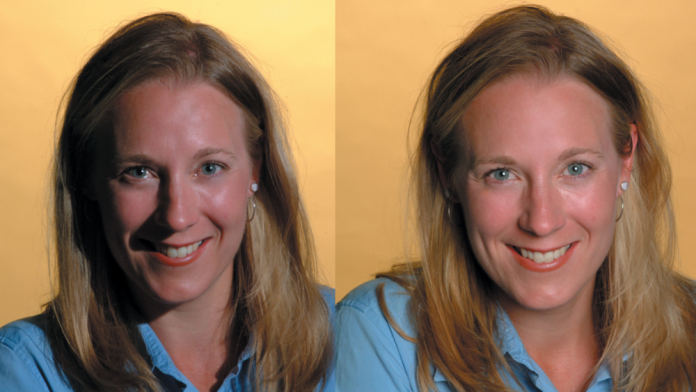
\includegraphics[width=12cm]{Obrazy/oswietlenieTwarzy.jpg}
        \caption{Przykład twarzy oświetlonej twardym (twarz po lewej) oraz miękkim światłem.~\cite{oswietlenieTwarzy}}
        \label{fig.oswietlenieTwarzy}
    \end{figure}
    W tym przypadku ryzyko utraty szczegółów oświetlanej twarzy jest większe.
    Kiedy twarz jest skierowana na wprost słońca, z dużym
    prawdopodobieństwem można stwierdzić, że zostanie oświetlona twardym światłem.
    Z kolei miękkie światło jest generowane na przykład przez zachmurzone niebo.
    Istotne jest także źródło światła, które
    może być punktowe lub rozproszone.
    Przy punktowym źródle światła cała twarz jest
    okryta jednolitym cieniem, którego intensywność zależy od "twardości" światła.
    Natomiast przy świetle rozproszonym intensywność cieni jest mniejsza.

    Na Rys \ref{fig.technikiWykrywaniaTwarzy} przedstawione są różne techniki wykrywania twarzy.
    \begin{figure}
        \centering
        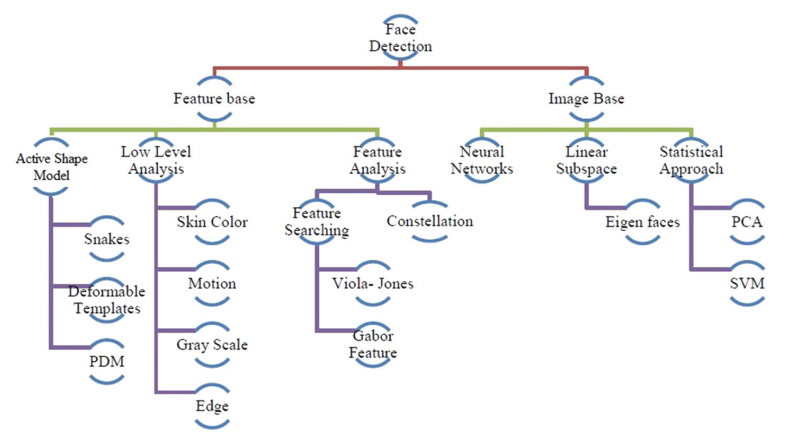
\includegraphics[width=15cm]{Obrazy/technikiWykrywaniaTwarzy.jpg}
        \caption{Różne techniki wykrywania twarzy.~\cite{faceDetectionTechniques}}
        \label{fig.technikiWykrywaniaTwarzy}
    \end{figure}
    %    https://sci-hub.tw/10.1007/s10462-018-9650-2

    %    Wyodrębnianie lub ekstrakcja cech polega na przekształceniu obrazu do zbioru zmiennych, które
    %    zostaną później użyte w wykrywaniu obiektu lub obiektów na obrazie.

    Jak widać metod wykrywania twarzy jest sporo.
    Omówienie każdej z nich zajęłoby dużo czasu.
    Poniżej zostaną przytoczone dwie metody wykrywania twarzy.
    Dodatkowo zostanie omówiona metoda, która posłużyła do wykrywania twarzy w niniejszej pracy.

    %https://sci-hub.tw/10.1016/S0031-3203(00)00134-5
    W pracy ,,An efficient algorithm for human face detection and facial
    feature extraction under different conditions''~\cite{wongLamSiu}
    przedstawiono opisaną w skrócie poniżej technikę wykrywania twarzy.
    W pierwszym etapie procesu obszary, gdzie może znajdować się ludzkie oko,
    są wykrywane przez przeprowadzenie testów na zacienionych rejonach obrazu.
    Pary takich obszarów wyodrębnia się na podstawie algorytmu genetycznego,
    aby następnie wyznaczyć możliwy obszar twarzy.
    Dla każdego obszaru mierzy się wartość dopasowania na podstawie jego projekcji na wektory własne,
    tzw. eigenfaces.
    Aby wiarygodność wykrywania była wyższa,
    każdy możliwy obszar twarzy normalizuje się pod kątem oświetlenia.
    Proces ten powtarza się pewną ilość razy,
    a następnie do dalszej weryfikacji są wybierane możliwe obszary twarzy o wysokiej wartości dopasowania.
    Na tym etapie mierzy się symetrię twarzy oraz sprawdza się,
    czy na każdym wybranym obszarze istnieją rysy twarzy.
    Rysy określa się przez ewaluację rzeźby topograficznej - wystających i wklęsłych elementów
    różnych regionów obszaru twarzy, poddanego uprzednio normalizacji.
    Algorytm jest w stanie wykryć także obszar twarzy, gdy głowa jest przechylona

    %todo Druga metoda wykrywania twarzy z https://www.researchgate.net/publication/334770252_An_Accurate_System_for_Face_Detection_and_Recognition
    %todo https://sci-hub.tw/10.1007/s10462-018-9650-2
    W roku 1997 w pracy pt. ,,Vision for man-machine interaction'' opisano metodę wykrywania twarzy bazującą na
    wykrywaniu cechy jaką jest kolor skóry~\cite{clowleyCoutaz}.
    Kolor skóry jest najbardziej widoczną cechą twarzy zarówno dla człowieka jak i dla maszyny.
    Ponadto kolor jest przetwarzany znacznie szybciej od innych cech.
    Przy dobrych warunkach oświetleniowych ustawienie twarzy nie ma wpływu na skuteczność wykrywalności twarzy
    opisywaną metodą.
    Każda metoda wykrywania twarzy posiada wady.
    Jedną z tych wad jest problem wykrywalności twarzy przy nierównomiernym oświetleniu.
    Problem pojawia się także, gdy na obrazie widoczny jest obszar skóry z poza twarzy np. z rąk.
    Warto zaznaczyć, że kolor twarzy na obrazie jest zależny od względnego kierunku oświetlenia.
    Obszar twarzy w omawianym algorytmie jest wykrywany poprzez normalizacje histogramu kolorów.
    Normalizacja jest potrzebna do redukcji wpływu luminancji na kolor.

    %todo trzecia metoda  - wstep do Haar Cascade https://drive.google.com/file/d/1nJ9S3HtuuFY6O1FLdIjRWSzWUFwZ_fuJ/view?usp=sharing
    Algorytm Haar Cascade jest najpopularniejszym algorytmem do wykrywania twarzy w bibliotece OpenCV. Właśnie ta
    biblioteka była jednym z niezbędnym elementów programu przy wykrywaniu wieku z tekstury twarzy.
    W związku z powyższym w wykrywaniu twarzy zastosowano algorytm Haar Cascade.
    Omawiany algorytm został zaprezentowany w książce ,,Rapid Object Detection using a Boosted Cascade of Simple
    Features'' w 2001 i składa się z trzech faz~\cite{violaJones}.
    W pierwszej obraz wejściowy przekształcany jest na obraz scałkowany.
    Następnie wykorzystywany jest algorytm do boostingu, który zmniejsza ilość klasyfikatorów tylko do tych
    najbardziej istotnych.
    W ostatniej fazie klasyfikatory łączone są w kaskady w celu przyspieszenia procesu wykrywania twarzy.
    Znaczna większość metod wykrywania obiektów na obrazie (w tym twarzy) wymaga wstępnego przekształcenia obrazu do
    skali szarości.

    %    https://towardsdatascience.com/face-recognition-with-opencv-haar-cascade-a289b6ff042a
    %    przez kogo został zaproponowany...
    %    byc moze cos o funkcji kaskadowej
    %    o tym ze OpenCv zawiera wytrenowane algorytmy Haar Cascade ktore wykrywaja ryj, oczy, usta itp
    %    wkleic obrazek z rodzajami filtrow
    %    jak dziala ten filtr
    %    przyklad na gebie emmy watson moze...
    %cosik tam jeszcze

    %    opisac jak dokladnie zaimplementowano to u nas
    %    przejscie na skale szarosci podczas wykrywania... czym ona jest?...
    \subsection{Konwersja do skali szarości oraz przestrzenie barw}\label{subsec:konwersja-do-skali-szarości-oraz-przestrzenie-barw}
    %todo https://sci-hub.tw/10.1007/s10462-018-9650-2
    Każdy piksel w trybie kolorowym ma określoną reprezentację barwy z określonego modelu.
    Najczęściej są to 3 lub 4 wartości~\cite{przestrzenieKolorow}.
    Pierwszą przestrzenią barw była CIEXYZ. Została ona stworzona w 1931 przez
    Międzynarodowa Komisja ds. Oświetlenia (International Commission on Illumination).
    Przestrzeń barw CIEXYZ została specjalnie stworzona, by odtworzyć sposób postrzegania barw przez ludzkie oko.
    Barwa jest opisywana w trzech współrzędnych trójchromatycznych X,Y,Z.
    Powyższe współrzędne są zależne od składowych - sprawności wizualnych czopków.
    Czopki to światłoczułe receptory siatkówki ludzkiego oka~\cite{przestrzenieKolorow}.
    Współrzędne X,Y,Z wyliczane są na podstawie trzech podstawowych barw R (czerwonej),
    G (zielonej) i B (niebieskiej).
    Współrzędne XYZ są często reprezentowane przez luminancję Y oraz współrzędne x, y chromatyczności.
    Wyliczanie współrzędnych x, y przedstawiono na wzorach \ref{wzor.chromX} oraz \ref{wzor.chromY}.
    \large
    \begin{equation}
        x = \frac{X}{X+Y+Z}
        \label{wzor.chromX}
    \end{equation}
    \normalsize

    \large
    \begin{equation}
        y = \frac{Y}{X+Y+Z}
        \label{wzor.chromY}
    \end{equation}
    \normalsize

    Na Rysunku~\ref{fig.CIEXYZ} przedstawiono diagram chromatyczności reprezentujący przestrzeń barw CIEXYZ.

    \begin{figure}
        \centering
        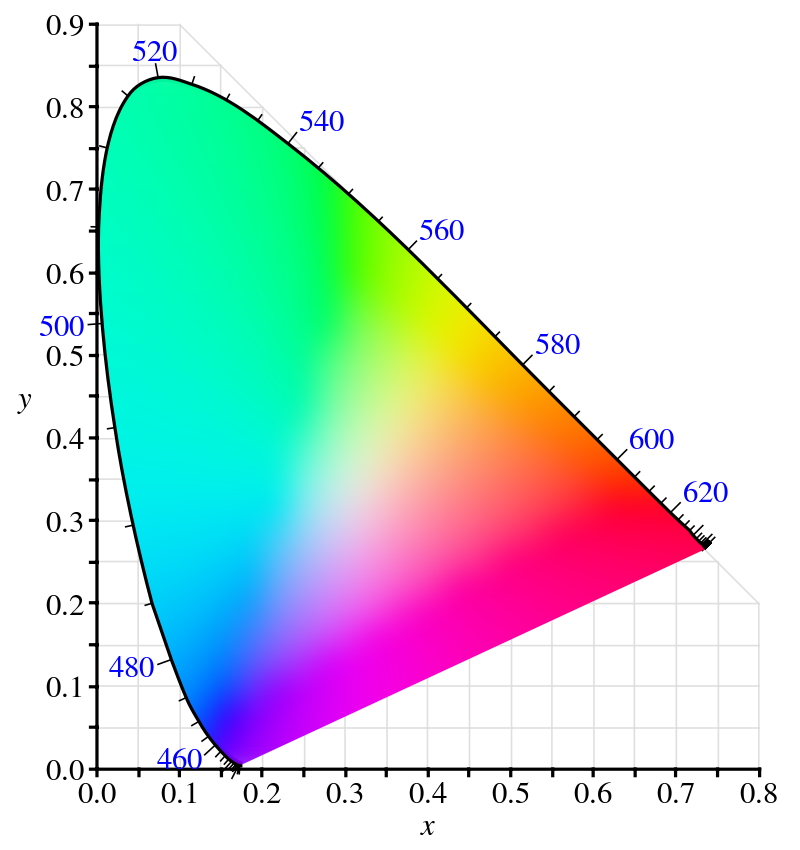
\includegraphics[width=6cm]{Obrazy/CIEXYZ.jpg}
        \caption{Przykład rozpoznawania obiektów na zdjęciu ulicy.~\cite{diagramCIEXYZ}}
        \label{fig.CIEXYZ}
    \end{figure}

    Kolory mogą byc także odwzorowane przez przestrzeń barw CMYK.
    Skrót CMYK oznacza odpowiednio:
    \begin{itemize}
        \item Cyan - odcień niebieskiego
        \item Magenta - kolor karmazynowy
        \item Yellow - kolor żółty
        \item K - key colour - kolor czarny
    \end{itemize}
    Barwa wynikowa powstaje poprzez mieszanie trzech kolorów - niebieskiego, karmazynowego oraz żółtego.
    Mieszanie zachodzi według zasady syntezy subtraktywnej~\cite{przestrzenieKolorow}.
    Synteza subtraktywna polega na mieszaniu kolorów przez odejmowanie promieniowań widzialnych różnych długości.
    Przykładem syntezy subtraktywnej jest np. mieszanie farb o różnych kolorach.

    Najczęściej barwy są reprezentowane przez przestrzeń barw RGB~\cite{przestrzenieKolorow}.
    Przestrzeń kolorów RGB składa się z trzech kanałów~\cite{kolory}:

    \begin{itemize}
        \item R - czerwonego (z angielskiego Red)
        \item G - zielonego (z angielskiego Green)
        \item B - niebieskiego (z angielskiego Blue)
    \end{itemize}
    Barwy mieszane są poprzez syntezę addytywną .
    W przeciwieństwie do syntezy subtraktywnej barwa wynikowa powstaje poprzez sumowanie wiązek światła widzialnego o
    różnych długościach~\cite{przestrzenieKolorow}.
    Każdy piksel opisany za pomocą przestrzenie barw RGB ma trzy 8-bitowe wartości reprezentujący każdy kanał.
    Spotykane
    są 12- lub 16-bitowe reprezentacje kanałów, jednak 8-bitowa jest najpopularniejsza.
    Dla 8-bitowych kanałów
    wartość ,,0''
    danego kanału oznacza brak jasności, natomiast ,,255'' maksymalną jasność.
    Poprzez mieszanie jasności tych trzech kanałów
    można uzyskać szerokie spektrum barw (Rysunek~\ref{fig.mieszanieKolorow}).

    \begin{figure}
        \centering
        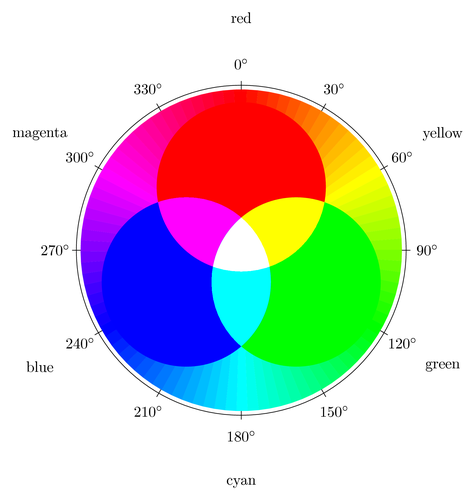
\includegraphics[width=7cm]{Obrazy/mieszanieKolorow.jpg}
        \caption{Mieszanie kanałów RGB~\cite{colorMixing}.}
        \label{fig.mieszanieKolorow}
    \end{figure}

    Przykładowo kolor o reprezentacji R=153 G=217 B=234 przedstawiono na Rysunku~\ref{fig.mieszanieKolorowBlekitny}

    \begin{figure}
        \centering
        
\includegraphics[width=2cm]{Obrazy/blekitny.jpg}
        \caption{Kolor R=153 G=217 B=234.}
        \label{fig.mieszanieKolorowBlekitny}
    \end{figure}

    Kolor (Rysunek~\ref{fig.mieszanieKolorowBlekitny}) może być też reprezentowany w kodzie szesnastkowym \#99D9EA.
    Każda
    wartość heksadecymalna odpowiada kolejno kanałowi R, G, B.

    Obraz może też być przedstawiony stosując odcienie jednej barwy.
    Taka obraz nazywa się obrazem monochromatycznym.
    Najczęściej stosowaną barwą w takich obrazach jest szarość~\cite{przestrzenieKolorow}.

    Istnieją 3 metody konwersji obrazu z przestrzeni RGB na monochromatyczny~\cite{colorMixing}.
    \begin{itemize}
        \item największej jasności
        \item średnia
        \item luminancji
    \end{itemize}
    Metoda największej jasności konwertuje na skalę szarości wg wzoru\ref{wzor.najwiekszaJasnosc}.

    \large
    \begin{equation}
        \frac{(max(R, G, B) + min(R, G, B))}{2}
        \label{wzor.najwiekszaJasnosc}
    \end{equation}
    \normalsize
    Metoda średnia bazuje na wzorze~\ref{wzor.metodaSrednia}, natomiast metodę luminancji ilustruje wzór~\ref{wzor.metodaLuminancji}.

    \large
    \begin{equation}
        \frac{(R + G + B)}{3}
        \label{wzor.metodaSrednia}
    \end{equation}
    \normalsize

    \large
    \begin{equation}
        0.21 R + 0.72 G + 0.07 B
        \label{wzor.metodaLuminancji}
    \end{equation}
    \normalsize

    W niniejszej pracy zastosowano konwersję za pomocą metody średniej.
    \subsection{Algorytm Haar Cascade}\label{subsec:algorytm-haar-cascade}

    Haar Cascade jest algorytmem służącym do wykrywania obiektów na obrazach.
    Został stworzony przez Paula Viola oraz Michaela Jonesa w 2001 roku~\cite{violaJones}.

    Opiera się na zbudowaniu kaskadowej funkcji za pomocą trenowania wielu zdjęć.
    Zdjęcia są dzielone na
    dwie kategorie - pozytywne oraz negatywne.
    Na zdjęciach klasyfikowanych jako pozytywne istnieje obiekt, który ma zostać wykryty, natomiast
    na zdjęciach negatywnych nie ma tego obiektu.

    Ekstrakcja cech w algorytmie Violi i Jonesa jest realizowana przez filtry Haara.
    Są to prostokątne okienka
    nakładane na obraz, które analizują jasność pikseli (Rysunek~\ref{fig.haarRectangles}).
    \begin{figure}
        \centering
        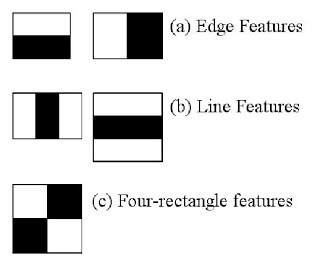
\includegraphics[width=7cm]{Obrazy/Haar_filter_rectangles.jpg}
        \caption{Filtr Haara a) krawędziowy b) liniowy c) szachownica~\cite{haar}}
        \label{fig.haarRectangles}
    \end{figure}

    Przed zastosowaniem filtru Haara obraz musi zostać przekształcony do skali szarości
    W niniejszej pracy należało przekształcić każdy obraz z trybu kolorowego na monochromatyczny co opisano w sekcji~\ref{subsec:konwersja-do-skali-szarości-oraz-przestrzenie-barw}.

    Każde okienko zawiera białe oraz czarne prostokąty.
    Wyznaczana jest suma jasności pikseli w obu rodzajach prostokątów, a
    następnie dla każdego okna obliczana jest różnica pomiędzy białymi a czarnymi.
    Opisywany algorytm ma zastosowanie w wykrywaniu krawędzi.
    Na granicy krawędzi istnieje różnica w jasności pikseli
    (Rysunek~\ref{fig.haarEmmaWatson}).

    \begin{figure}
        \centering
        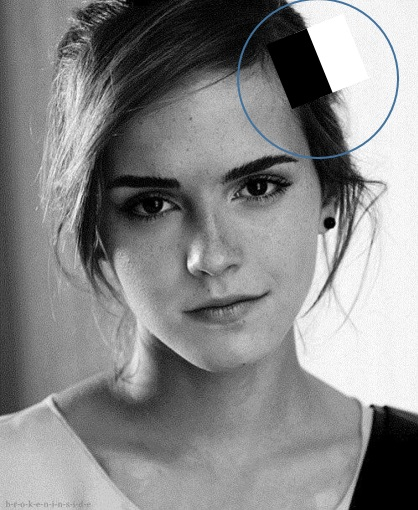
\includegraphics[width=6cm]{Obrazy/haarEmmaWatson.jpg}
        \caption{Filtr Haara nałożony na krawędź twarzy~\cite{haar}}
        \label{fig.haarEmmaWatson}
    \end{figure}

    W celu poprawy efektywności sumowania pikseli stosowane są
    rozwiązanie zwane w języku angielskim Summed-area table~\cite{violaJonesRealTimeOb}.Summed-area table jest również
    nazywana w literaturze Integral Image, czyli obrazem scałkowanym.
    Ideą obrazu scałkowanego jest,
    aby każdy obraz
    został
    przekształcony w
    tabelę, w której każdy element x,y tej tabeli odpowiada sumie jasności wszystkich pikseli według wzoru~\ref{wzor.summedAreaTable}.

    \large
    \begin{equation}
        I(x,y) = \sum_{{x}'\leq x \cap {y}'\leq y}^{} i({x}',{y}')
        \label{wzor.summedAreaTable}
    \end{equation}
    \normalsize
    gdzie I(x,y) jest wartością na pozycji x,y w tabeli(tabela obrazu scałkowanego), i(x,y) - jasność piksela o
    współrzędnych x,y na obrazie.

    Na Rysunku~\ref{fig.przedCalkowaniem} przedstawiona jest tabela prezentująca jasność pikseli przed
    zastosowaniem całkowania obrazu.
    \begin{figure}
        \centering
        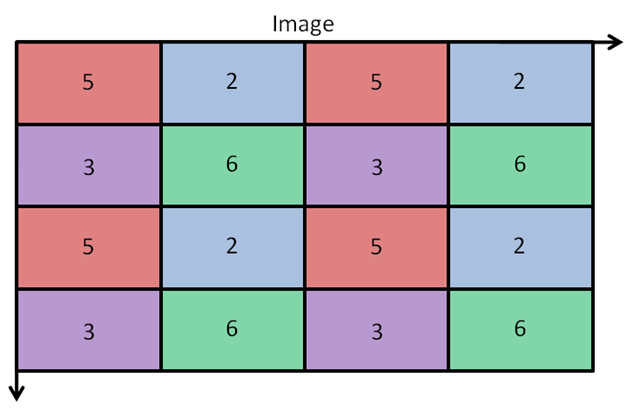
\includegraphics[width=6cm]{Obrazy/przedCalkowaniem.jpg}
        \caption{Tabela jasności poszczególnych pikseli przed zastosowaniem całkowania~\cite{integralImages}}
        \label{fig.przedCalkowaniem}
    \end{figure}

    Po całkowaniu otrzymujemy tabelę podobną do przedstawionej na Rysunku~\ref{fig.poCalkowaniu}.
    \begin{figure}
        \centering
        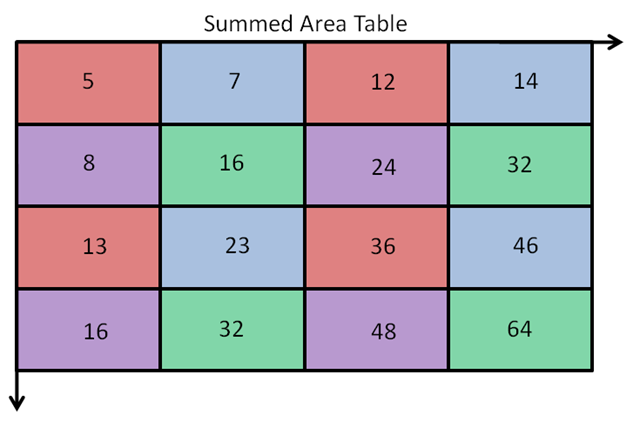
\includegraphics[width=6cm]{Obrazy/poCalkowaniu.jpg}
        \caption{Filtr Haara nałożony na krawędź twarzy~\cite{integralImages}}
        \label{fig.poCalkowaniu}
    \end{figure}

    Sumowanie przykładowego okna (Rysunek~\ref{fig.sumowanieOkna}) wymaga 4 operacji (Wzór~\ref{wzor.windowsSum}).
    \begin{figure}
        \centering
        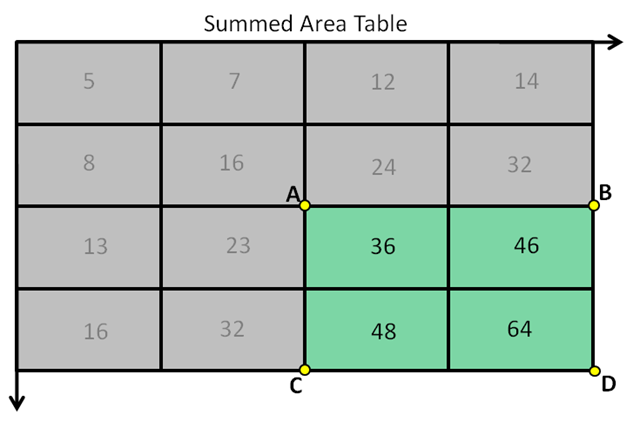
\includegraphics[width=6cm]{Obrazy/sumowanieOkna.jpg}
        \caption{Sumowanie okna~\cite{integralImages}}
        \label{fig.sumowanieOkna}
    \end{figure}


    \large
    \begin{equation}
        \sum_{x_0\leq x \leq x_1\cap {y}\leq y \leq y_1}^{} i(x,y) = I(D) + I(A) - I(B) - I(C)
        \label{wzor.windowsSum}
    \end{equation}
    \normalsize
    gdzie lewa część równania oznacza sumę jasności pikseli
    zaznaczonego okna tj.
    na Rysunku~\ref{fig.sumowanieOkna}, I(A) - wartość scałkowanego obrazu przy punkcie A
    (analogicznie I(B), I(C), I(D)) - (Rysunek~\ref{fig.sumowanieOkna}).

    W związku z powyższym obliczenie wartości dla krawędziowego filtru Haara wymaga obliczenia różnicy dwóch sum co
    wymaga ośmiu operacji.
    Reprezentacja obrazu za pomocą obrazu scałkowanego znacznie zwiększa efektywność obliczania wartości w filtrze
    Haara.


    Liczba cech wykrywanych w zdjęciu za
    pomocą filtru Haara jest znacznie większa od liczby pikseli na obrazie~\cite{violaJones}.
    Dla obrazu o rozmiarze 384x288 liczba cech wynosi ponad 180000.
    Autorzy algorytmu stwierdzili, że dla zwiększenia szybkości algorytmu należy wybrać małą grupę cech,
    które razem mogą stworzyć jeden efektywny klasyfikator obiektu.
    W celu wyodrębnienia tych istotnych cech zastosowano algorytm Adaboost, który został opisany poniżej.

    Zbiór n obrazów do trenowania można oznaczyć tak jak we wzorze~\ref{wzor.zbiorTrenujacy}:
    \large
    \begin{equation}
        (x_1, y_1), (x_2, y_2), \ldots, (x_n, y_n)
        \label{wzor.zbiorTrenujacy}
    \end{equation}
    \normalsize

    oznacza, że obraz jest odpowiednio negatywny lub pozytywny.
    Następnym krokiem jest inicjalizacja wag (Wzór~\ref{wzor.wagi}).

    \large
    \begin{equation}
        w_{1,i} = \frac{1}{2m}, \frac{1}{2l}
        \label{wzor.wagi}
    \end{equation}
    \normalsize
    odpowiednio dla $y_i = 0, 1$
    , gdzie m, l oznacza odpowiednio liczbę negatywnych oraz pozytywnych zdjęć.
    Następnie
    Dla t = 1, \ldots, T:

    1. Normalizowane są wagi (Wzór~\ref{wzor.adaboost1}):
    \large
    \begin{equation}
        w_{t,i} = \frac{w_{t,i}}{\sum_{j=1}^{n}w_{t,j}}
        \label{wzor.adaboost1}
    \end{equation}
    \normalsize
    $w_{t}$ jest rozkładem prawdopodobieństwa

    2. Dla każdej cechy j, trenowany jest klasyfikator $h_{j}$, który używa tylko jedną cechę wyliczoną z filtru Haara.
    Błąd jest wyliczony następująco (Wzór~\ref{wzor.adaboost2}):
    \large
    \begin{equation}
        w_{t}, \epsilon_{j} = \sum_{i}^{}w_{i} \abs{h_{j}(x_{i}) - y_{i}}
        \label{wzor.adaboost2}
    \end{equation}
    \normalsize

    3. Wybierany jest klasyfikator $h_{t}$ z najmniejszym błędem \epsilon_{t}.

    4. Następuje aktualizacja wag (Wzór~\ref{wzor.adaboost3}):
    \large
    \begin{equation}
        w_{t+1,i} = w_{t,i}\beta_{t}^{1-e_{i}}
        \label{wzor.adaboost3}
    \end{equation}
    \normalsize
    , gdzie $e_{i} = 0$. Jeśli $x_{i}$ jest sklasyfikowane prawidłowo, wtedy $e_{i}=1$,
    w innym wypadku $\beta_{t} = \frac{\epsilon_{t}}{1 - \epsilon_{t}}$.

    Silny klasyfikator $h(x)$ jest opisany równaniem:
    \large
    \begin{equation}
        h(x) = \left\{ \begin{array}{ll}
                           1 & \textrm{gdy $\sum_{t=1}^{T}\alpha_{t}h_{t}(x) >= \frac{1}{2} \sum_{t=1}^{T}\alpha_{t}$}\\
                           0 & \textrm{w przeciwnym wypadku}\\
        \end{array} \right.
        \label{wzor.adaboost4}
    \end{equation}
    \normalsize
    , gdzie $\alpha_{t} = \lg \frac{1}{\beta_{t}}$

    Algorytm Adaboost zmniejsza ilość cech Haara z ponad stu tysięcy do kilkuset - do tych najistotniejszych cech.

    Ostatnim etapem jest wytworzenie kaskady klasyfikatorów.
    Zwiększa ona znacznie szybkość wykrywania pożądanego obiektu na obrazie.
    Ideą kaskady jest zgrupowanie klasyfikatorów,
    które powstały w poprzednim procesie - procesie boostingu.
    Klasyfikatory są grupowane w okna.
    Okna są połączone ze sobą tak jak na rysunku~\ref{fig.kaskadaHaar}.
    \begin{figure}
        \centering
        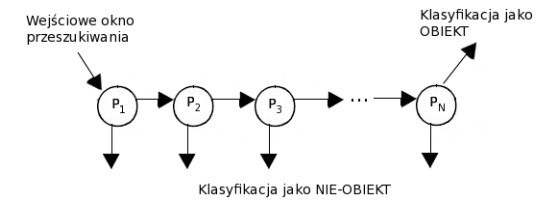
\includegraphics[width=11cm]{Obrazy/kaskadaHaar.jpg}
        \caption{Kaskada klasyfikatorów.~\cite{kaskadaHaarObraz}}
        \label{fig.kaskadaHaar}
    \end{figure}
    Okna są oznaczone jako P1, P2, \ldots, Pn.
    Gdy dane okno wykryje obiekt przechodzi do kolejnego okna w kaskadzie.
    W przeciwnym wypadku algorytm przerywa działanie i na danym obrazie nie zostaje zidentyfikowany obiekt.
    Okna są poustawiane tak aby każde z nich klasyfikowało obiekt z różnym prawdopodobieństwem wykrycia oraz
    prawdopodobieństwem błędu.
    Składnikami wyżej wymienionego prawdopodobieństwa jest macierz pomyłek (Rysunek~\ref{fig.ConfusionMatrix}).

    \begin{figure}
        \centering
        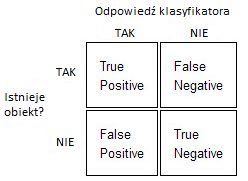
\includegraphics[width=11cm]{Obrazy/ConfusionMatrix.jpg}
        \caption{Macierz pomyłek.}
        \label{fig.ConfusionMatrix}
    \end{figure}

    Z macierzy\ref{fig.ConfusionMatrix} można odczytać czy klasyfikator poprawnie sklasyfikował dane testowe.
    W macierzy użyto 4 pojęcia:
    \begin{itemize}
        \item TP (true positive) - poprawna klasyfikacja, jako obiekt
        \item TN (true negative) - poprawna klasyfikacja, jako nie - obiekt
        \item FP (false positive) - błędna klasyfikacja jako obiekt
        \item FN (false negative) - błędna klasyfikacja jako nie - obiekt
    \end{itemize}

    Prawdopodobieństwo błędu wyliczane jest ze współczynnika FPR (false positive rate) (Wzór~\ref{wzor.fpr}).

    \large
    \begin{equation}
        FPR= \frac{FP}{FP+TN}
        \label{wzor.fpr}
    \end{equation}
    \normalsize

    Natomiast prawdopodobieństwo wykrycia obiektu wyliczane jest ze współczynnika TPR (true positive ratio)
    (Wzór~\ref{wzor.tpr})
    \large
    \begin{equation}
        TPR= \frac{TP}{TP+FN}
        \label{wzor.tpr}
    \end{equation}
    \normalsize

    Pierwsze okna posiadają klasyfikatory o słabszym TPR oraz FPR niż kolejne okna.
    Oznacza to, że prawdopodobieństwo TPR w oknie $P_{x-1}$ jest mniejsze od tego w $P_{x}$.
    Natomiast prawdopodobieństwo FPR w oknie $P_{x-1}$ jest większe od tego w $P_{x}$.
    Ostatnie okna mają największy współczynnik TPR oraz najmniejszy FRP ze wszystkich.
    Takie ustawienie okien ma na celu wstępne przepuszczenie przez okna obrazy,
    które z dużym prawdopodobieństwem zawierają szukany obiekt.
    Natomiast ostatnie okna w kaskadzie analizują niewielką część obrazu wejściowego.
    %Opis kaskady
    %    The overall form of the detection process is that of a degenerate decision tree, what we call a “cascade” (see Figure 4). A positive result from the first classifier triggers the
    %    evaluation of a second classifier which has also been adjusted to achieve very high detection rates. A positive result
    %    from the second classifier triggers a third classifier, and so
    %    on. A negative outcome at any point leads to the immediate
    %    rejection of the sub-window.
    %    Stages in the cascade are constructed by training classifiers using AdaBoost and then adjusting the threshold to
    %    minimize false negatives. Note that the default AdaBoost
    %    threshold is designed to yield a low error rate on the training data. In general a lower threshold yields higher de
    %    W ostatniej fazie stosowany jest algorytm kaskady klasyfikatorów.
    %    Klasyfikatory są podzielone na grupy i
    %    połączone ze sobą kaskadowo.
    %    W algorytmie każda grupa może podjąć dwie decyzje - przekazanie danych z klasyfikatorów
    %    do kolejnej grupy lub ich odrzucenie.
    %    Ma to na celu odrzucenie wielu negatywnych danych z klasyfikatorów~\cite{cascade}.

    Biblioteka OpenCV zawiera wytrenowane klasyfikatory, które zostały użyte w tej pracy magisterskiej.
    Wykorzystano
    je do wykrycia twarzy, ust oraz oczu.
    Klasyfikatory mają postać plików xml, które można znaleźć na oryginalnym
    repozytorium projektu OpenCv.

    %1600 wyrazow
    \section{Wyznaczanie stref}\label{sec:wyznaczanieStref}
    %Wzory na wyznaczenie stref z "okienek"
    Przed wyznaczeniem stref zmarszczkowych należy zidentyfikować na twarzy oczy oraz nos
    (Rysunek~\ref{fig.wykrywanieOczuNosa}).
    \begin{figure}
        \centering
        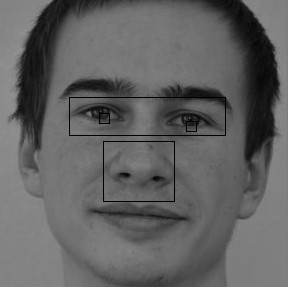
\includegraphics[width=8cm]{Obrazy/wykrywanieOczuNosa.jpg}
        \caption{Wykryty nos oraz oczy.}
        \label{fig.wykrywanieOczuNosa}
    \end{figure}


    Należy podkreślić, że algorytm przerywa działanie jeśli nie zostanie wykryta twarz, oczy lub nos.

    Gdy zostanie wykryty obszar twarzy oczu oraz nosa wyznaczone zostaje sześć stref zmarszczkowych
    (Rysunek~\ref{fig.wykrywanieStrefZmarszczkowych}).

    \begin{figure}
        \centering
        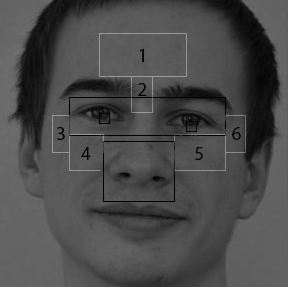
\includegraphics[width=8cm]{Obrazy/strefyZmarszczkowe.jpg}
        \caption{Strefy zmarszczkowe widoczne w białych prostokątach.}
        \label{fig.wykrywanieStrefZmarszczkowych}
    \end{figure}

    Strefy zmarszczkowe są na czole (Strefa ,,1''), w górnej części nosa (Strefa ,,2''), górnej części policzków
    (Strefa ,,4'' i ,,5'') oraz w okolicach powiek (Strefa ,,3'' i ,,6'').
    To właśnie te miejsca zostały uznane przez autorów książki ,,Age Estimation from Face Image using Wrinkle
    Features''~\cite{wrinkleFeatures} za najbardziej znaczące w detekcji wieku.

    Po detekcji oczu należy zmierzyć odległość pomiędzy środkiem lewego oka ($x_{l},y_{l}$),
    a prawego ($x_{p},y_{p}$)
    (Wzór~\ref{wzor.odlegloscPomiedzyOczami}).
    \large
    \begin{equation}
        d= \sqrt{\left ( x_{r} - x_{l} \right )^{2}+\left (y_{r} - y_{l}  \right )^{2}}
        \label{wzor.odlegloscPomiedzyOczami}
    \end{equation}
    \normalsize

    Odległość d służy do wyznaczanie strefy znajdującej się na czole (Rysunek~\ref{fig.wyznaczenieCzola}).


    \begin{figure}
        \centering
        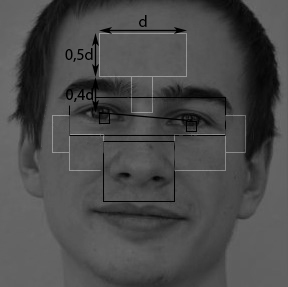
\includegraphics[width=11cm]{Obrazy/wyliczenieCzolka.jpg}
        \caption{Wyznaczenie strefy znajdującej się na czole.}
        \label{fig.wyznaczenieCzola}
    \end{figure}

    Autorzy~\cite{wrinkleFeatures} algorytmu założyli, że odległość od linii oczy do linii brwi wynosi $0,4 * d$.
    Natomiast wymiary ,,strefy czoła'' wynoszą $d \times 0,5d$.

    Na Rysunku~\ref{fig.wspolrzedneDoWyliczeniaStref} przedstawione są współrzędne, które są pomocne w wyznaczaniu
    stref zmarszczkowych.

    \begin{figure}
        \centering
        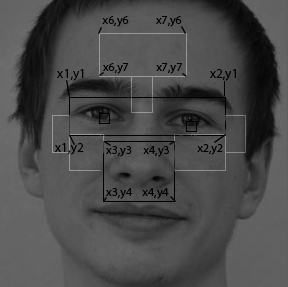
\includegraphics[width=9cm]{Obrazy/wspolrzedneDoWyliczeniaStref.jpg}
        \caption{Pomocnicze współrzędne do wyliczania stref zmarszczkowych.}
        \label{fig.wspolrzedneDoWyliczeniaStref}
    \end{figure}

    Strefa 2 została wyznaczona znając położenie prawego oka, dystansu między oczami oraz strefy ,,1''.
    Każda strefa może być wyznaczona przez jeden punkt (Rysunek~\ref{fig.wykrywanieStrefZmarszczkowychPunkty})
    oraz jej wymiary.

    \begin{figure}
        \centering
        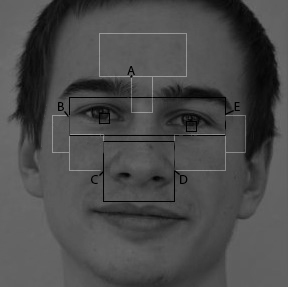
\includegraphics[width=8cm]{Obrazy/wykrywanieStrefZmarszczkowychPunkty.jpg}
        \caption{Punkty wyznaczające położenie stref.}
        \label{fig.wykrywanieStrefZmarszczkowychPunkty}
    \end{figure}

    Współrzędna x punktu A została wyznaczona ze wzoru~\ref{wzor.punktXA}

    \large
    \begin{equation}
        x_{A}=x_{6} + 0,375 \times d
        \label{wzor.punktXA}
    \end{equation}
    \normalsize
    , gdzie $x_{6}$ to współrzędna z Rysunku~\ref{fig.wspolrzedneDoWyliczeniaStref}.
    Natomiast $d$ jest odległością pomiędzy oczami (Wzór~\ref{wzor.odlegloscPomiedzyOczami}).

    Współrzędna y punktu A - Wzór~\ref{wzor.punktYA}:

    \large
    \begin{equation}
        y_{A}=y_{7}
        \label{wzor.punktYA}
    \end{equation}
    \normalsize
    Współrzędna $y_{7}$ analogicznie jak $x_{6}$ znajduje się na Rysunku~\ref{fig.wspolrzedneDoWyliczeniaStref}.

    Zakładając, że prawe oko ma współrzędne $x_{o}$ oraz  $y_{o}$ wyznaczana jest wysokość strefy 2
    (Wzór~\ref{wzor.punktHA}).
    \large
    \begin{equation}
        h_{A}=y_{o}-y_{7}
        \label{wzor.punktHA}
    \end{equation}
    \normalsize

    Szerokość strefy 2 (Wzór~\ref{wzor.punktWA}):
    \large
    \begin{equation}
        w_{A}=0,25 * d
        \label{wzor.punktWA}
    \end{equation}
    \normalsize
    Wartość 0,25 ze wzoru~\ref{wzor.punktWA} została dobrana empirycznie.

    Współrzędne punktu C (strefa 4) zostają wyznaczone ze Wzoru~\ref{wzor.punktXC} oraz~\ref{wzor.punktYC}.
    \large
    \begin{equation}
        x_{C}=x_{3}
        \label{wzor.punktXC}
    \end{equation}
    \normalsize

    \large
    \begin{equation}
        y_{C}= \frac{y_{4} - y_{3}}{2}
        \label{wzor.punktYC}
    \end{equation}
    \normalsize

    Wysokość oraz szerokość strefy 4 (Wzór~\ref{wzor.punktHC} oraz~\ref{wzor.punktWC})

    \large
    \begin{equation}
        h_{C}=y_{C} - y_{3}
        \label{wzor.punktHC}
    \end{equation}
    \normalsize

    \large
    \begin{equation}
        w_{C}= x_{3} - x_{1}
        \label{wzor.punktWC}
    \end{equation}
    \normalsize

    Strefa 5 zawiera punkt D - Wzór~\ref{wzor.punktXD} oraz~\ref{wzor.punktYD}.

    \large
    \begin{equation}
        x_{D}=x_{4}
        \label{wzor.punktXD}
    \end{equation}
    \normalsize

    \large
    \begin{equation}
        y_{D}= y_{C}
        \label{wzor.punktYD}
    \end{equation}
    \normalsize

    Dla strefy 5 wyznaczamy wysokość (Wzór~\ref{wzor.punktHD}) oraz szerokość (Wzór~\ref{wzor.punktWD}).

    \large
    \begin{equation}
        h_{D}=h_{C}
        \label{wzor.punktHD}
    \end{equation}
    \normalsize

    \large
    \begin{equation}
        w_{D}= x_{2} - x_{4}
        \label{wzor.punktWD}
    \end{equation}
    \normalsize

    Strefa 3 zawiera punkt B wyznaczany ze Wzorów~\ref{wzor.punktXB} i~\ref{wzor.punktYB}

    \large
    \begin{equation}
        x_{B}=x_{1}
        \label{wzor.punktXB}
    \end{equation}
    \normalsize

    \large
    \begin{equation}
        y_{B}= \frac{y_{2} - y_{1}}{2}
        \label{wzor.punktYB}
    \end{equation}
    \normalsize

    Wysokość (Wzór~\ref{wzor.punktHB}) oraz szerokość (Wzór~\ref{wzor.punktWB}) strefy 3.

    \large
    \begin{equation}
        h_{B}=y_{C} - y_{B}
        \label{wzor.punktHB}
    \end{equation}
    \normalsize

    \large
    \begin{equation}
        w_{B}= w_{C} * 0,4
        \label{wzor.punktWB}
    \end{equation}
    \normalsize

    Na samym końcu zostaje wyznaczona strefa 6.
    Wyznaczona zostaje współrzędna E - Wzór~\ref{wzor.punktXE} i~\ref{wzor.punktYE}.
    \large
    \begin{equation}
        x_{E}=x_{2}
        \label{wzor.punktXE}
    \end{equation}
    \normalsize

    \large
    \begin{equation}
        y_{E}= y_{B}
        \label{wzor.punktYE}
    \end{equation}

    Szerokość oraz wysokość strefy 6.

    \large
    \begin{equation}
        h_{E}=h_{B}
        \label{wzor.punktHE}
    \end{equation}
    \normalsize

    \large
    \begin{equation}
        w_{E}= w_{D} * 0,4
        \label{wzor.punktWE}
    \end{equation}
    \normalsize

    Należy zauważyć, że szerokość strefy 3 i 6 jest pomnożona przez 0,4 razy szerokość odpowiednio
    strefy 4 i 5.
    Wartość ,,0,4'' została dobrana empirycznie.
    \section{Wykrywanie zmarszczek - detektor Canny}\label{sec:wykrywanie-zmarszczek---detektor-canny}
    %todo opis detektora z wiki angielskiej
    %moze troche opisu configu Cannego od Anielskiej
    Następnym krokiem algorytmu po wyznaczeniu stref zmarszczkowych jest wyodrębnienie zmarszczek.
    W celu identyfikacji zmarszczek zastosowano detektor Canny.
    Detekcja krawędzi pozwala na wyodrębnienie wielu użytecznych cech z obrazu.
    Ponadto znacznie zmniejsza ilość informacji do przetworzenia przez algorytm,
    który wyodrębnia cechy z obrazu.
    Istnieje wiele detektorów krawędzi,
    jednak detektor Canny jest jednym z najbardziej dokładnych i niezawodnych.
    Metoda detekcji została opracowana przez Johna F. Canny w 1986 roku.
    Oprócz samej implementacji algorytmu Canny zaprezentował teorię obliczeniową,
    która wyjaśnia działanie tej metody. Canny ponadto zauważył,
    że wymagania dotyczące implementacji detekcji krawędzi są podobne do siebie w wielu systemach wizyjnych.
    W związku z powyższym jego algorytm może zostać zastosowany w wielu systemach wizyjnych.
    Najważniejsze zasady,
    które są niezbędne do dobrej detekcji krawędzi w opisywanym algorytmie są przedstawione poniżej:
    \begin{itemize}
        \item Detekcja krawędzi z niskim prawdopodobieństwem błędu:
        Oznacza to, że algorytm powinien wykryć jak najwięcej krawędzi, które rzeczywiście istnieją.
        Natomiast ilość krawędzi wykrytych błędnie powinna być jak najmniejsza.
        \item Precyzja detekcji: Algorytm powinien precyzyjnie zlokalizować krawędź
        \item Brak redundantnych detekcji:
        Krawędź powinna być zlokalizowana jednokrotnie.
        Szum na obrazie nie powinien generować dodatkowych krawędzi.
    \end{itemize}
    W algorytmie detekcji Canny używa rachunku wariacyjnego.
    Rachunek wariacyjny to dziedzina analizy matematycznej.
    Dziedzina ta analizuje przestrzenie funkcyjne i znajduje w nich ekstrema funkcjonałów.
    Funkcjonały natomiast odwzorowują przestrzeń wektorową na liczby rzeczywiste.
    Reasumując, rachunek wariacyjny pomaga znaleźć charakterystyczną funkcję.
    Funkcjonał dla powyższej funkcji przyjmuje wartość ekstremalną.
    Algorytm detektora jest podzielony na kilka kroków~\cite{Canny}:
    \begin{itemize}
        \item Redukcja szumów na obrazie filtrem Gaussa.
        \item Szukanie gradientów jasności.
        \item Zastosowanie techniki pocieniania krawędzi.
        \item Likwidacja krawędzi o małym gradiencie jasności.
        \item Filtracja poprzez histerezę.
    \end{itemize}
    \subsection{Redukcja szumów na obrazie filtrem Gaussa}\label{subsec:redukcja-szumów-na-obrazie-filtrem-gaussa}
    Szum na obrazie to piksele o losowym kolorze, jasności oraz umiejscowieniu (współrzędnych na obrazie).
    Powyższe piksele są nadmiarowymi informacjami o obrazie oraz są efektem ubocznym przetwarzania obrazu
    przez matrycę cyfrową (Rysunek~\ref{fig.lenkaSzumy}).

    \begin{figure}
        \centering
        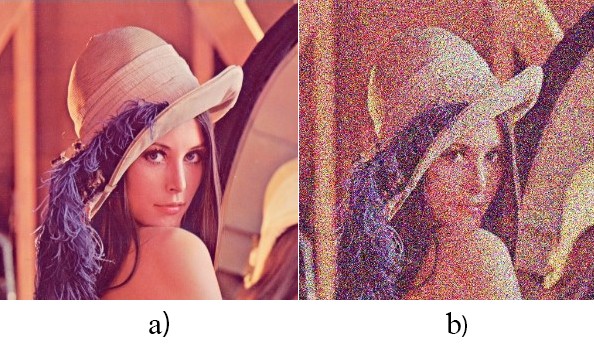
\includegraphics[width=11cm]{Obrazy/lenkaSzumy.jpg}
        \caption{a) Obraz z nieznaczną ilością szumów b) Obraz ze znaczną ilością szumu.~\cite{lenkaSzumy}}
        \label{fig.lenkaSzumy}
    \end{figure}

    Efekt szumu jest spotykany również w fotografii analogowej.
    W fotografii cyfrowej szum wzrasta na skutek zwiększania czułości matrycy lub przez wzrost jej temperatury.
    Redukcję szumów można uzyskać stosując filtr Gaussa.
    Splot filtru Gaussa z obrazem daje w wyniku wygładzony obraz ze zmniejszoną ilością szumu.
    Filtr Gaussa może mieć różne wymiary.
    Najczęściej stosowanym jest 5x5.
    Rozmiar filtra ma wpływ na wydajność wygładzania obrazu, a co za tym idzie na czułość wykrywania szumu~\cite{Canny}.
    \subsection{Szukanie gradientów jasności}\label{subsec:szukanie-gradientów-jasności}
    Istotnym parametrem w wykrywaniu krawędzi jest gradient jasności.
    Określa on jak bardzo zmienia się jasność danego piksela względem sąsiadujących pikseli.
    Gradient jasności otrzymany zostaje ze wzoru~\ref{wzor.gradientJasnosci}:
    \large
    \begin{equation}
        G = \sqrt{G_{x}^{2} + G_{y}^{2}}
        \label{wzor.gradientJasnosci}
    \end{equation}
    \normalsize
    gdzie Gx jest zmianą jasności danego piksela w kierunku poziomym, a Gy w kierunku pionowym
    Kierunek gradientu opisuje wzór~\ref{wzor.kierunekGradientu}
    \large
    \begin{equation}
        \Theta = atan2(G_{y}, G_{x})
        \label{wzor.kierunekGradientu}
    \end{equation}
    \normalsize
    Krawędzie na obrazie charakteryzują się pewną zmianą jasności na danym obszarze obrazu.
    Krawędź na obrazie może być położona pod różnym kątem.
    Opisywany detektor używa 4 filtry w celu wykrycia pionowych, poziomych, ukośnych krawędzi.

    Kierunek jest zaokrąglony do jednego z filtrów kierunku: poziomego ($\Theta = 0^{\circ}$),
    pionowego($\Theta = 90^{\circ}$) lub ukośnego ($\Theta = 45^{\circ}$
    lub $\Theta = 135^{\circ}$ stopni).
    Każdy piksel obrazu otrzymuje wartość gradientu (Wzór~\ref{wzor.gradientJasnosci})
    oraz kierunek - zgodny z powyższym filtrem kierunku.
    W wyniku powyższego działania zostaje otrzymany obraz gradientowy~\cite{Canny}.
    \subsection{Zastosowanie techniki pocieniania krawędzi}\label{subsec:zastosowanie-techniki-pocieniania-krawędzi}
    Pocienianie krawędzi służy do filtracji krawędzi powstałych po poprzednim kroku.
    Krawędzie wykryte za pomocą gradientu są rozmyte (nieostre).
    Technika pocienianie krawędzi szuka na małym obszarze gradientów o największej wartości.
    Wszystkie mniejsze są ignorowane.
    Dzięki temu zostawiane są gradienty o największej wartości, które identyfikują najostrzejsze krawędzie.
    Algorytm operuje na obrazie gradientowym powstałym przez algorytm opisany w sekcji~\ref{subsec:szukanie-gradientów-jasności}
    Działa on następująco.

    Odczytana zostaje wartość gradientu oraz jego kierunek dla danego piksela.
    Następnie wartość gradientu zostaje porównana z wartościami gradientu dla
    dwóch sąsiednich pikseli.
    Pierwszy sąsiedni piksel jest wyznaczony przed aktualny kierunek gradientu, a drugi przez przeciwny kierunek.
    Jeśli wartość danego piksela jest największa spośród pikseli wzdłuż wyżej wymienionych linii,
    to dany piksel należy do najostrzejszej krawędzi~\cite{Canny}.

    \subsection{Filtracja krawędzi o małym gradiencie jasności}\label{subsec:filtracja-krawędzi-o-małym-gradiencie-jasności}
    Zastosowanie techniki pocieniania krawędzi zostawia wiele krawędzi, które są wygenerowane przez szum i zmiany
    kolorów na obrazie.
    Kolejnym krokiem jest filtracja powyższych krawędzi, gdyż są one nadmiarowe.
    W tym celu ustawiany jest pewien próg - próg mały.
    Oprócz progu małego ustawiany jest próg duży w celu wyodrębnienia krawędzi o wysokim gradiencie jasności.
    Jeśli wartość gradientu dla danej krawędzi jest mniejsza od progu małego, to zostaje ona usunięta.
    W przypadku, gdy wartość jest większa od progu małego, ale mniejsza od progu dużego to dana krawędź
    zostaje oznaczona jako słaba.
    Krawędź zostaje oznaczona jako mocna, gdy wartość gradientu dla niej jest większa od wartości progu dużego~\cite{Canny}.

    \subsection{Filtracja poprzez histerezę}\label{subsec:filtracja-poprzez-histerezę}
    W wyniku działania algorytmu do tej pory zostały uzyskane słabe oraz mocne krawędzie.
    Mocne krawędzie zostaną oznaczone jako prawdziwe krawędzie znajdujące się na obrazie.
    Słabe krawędzie mogą być częścią mocnych krawędzi.
    Ponadto mogą zostać wygenerowane przez szum lub zmiany kolorów.
    Powyższe krawędzie nie są prawdziwymi krawędziami w obrazie, więc w ostatnim kroku algorytmu powinny zostać
    przefiltrowane.
    Słabe krawędzie, które są powiązane z mocnymi znajdują się w najbliższym sąsiedztwie z mocnymi krawędziami.
    W celu odnalezienia tych powiązań pomiędzy krawędziami zostaje zastosowana analiza spójności krawędzi.
    Jeśli zostaje zidentyfikowane powiązanie pomiędzy mocną, a słabą krawędzią to słaba krawędź zostaje w obrazie.
    W przypadku, gdy słaba krawędź nie jest powiązana z żadną mocną krawędzie - zostaje usunięta~\cite{Canny}.

    \section{Wyliczanie wrinkle feature}\label{sec:wyliczanieWrinkleFeature}
    W wyniku działania detektora Cannego, który został opisany w sekcji~\ref{sec:wykrywanie-zmarszczek---detektor-canny}
    wygenerowany zostaje obraz binarny z wyodrębnionymi krawędziami.
    Obraz binarny zawiera piksele o dwóch wartościach jasności pikseli.
    Piksel może być albo biały albo czarny.
    Krawędzie można rozpoznać jako białe piksele, natomiast czarne piksele oznaczają brak krawędzi (Rysunek~\ref{fig.mojaTwarzGray}).

    \begin{figure}
        \centering
        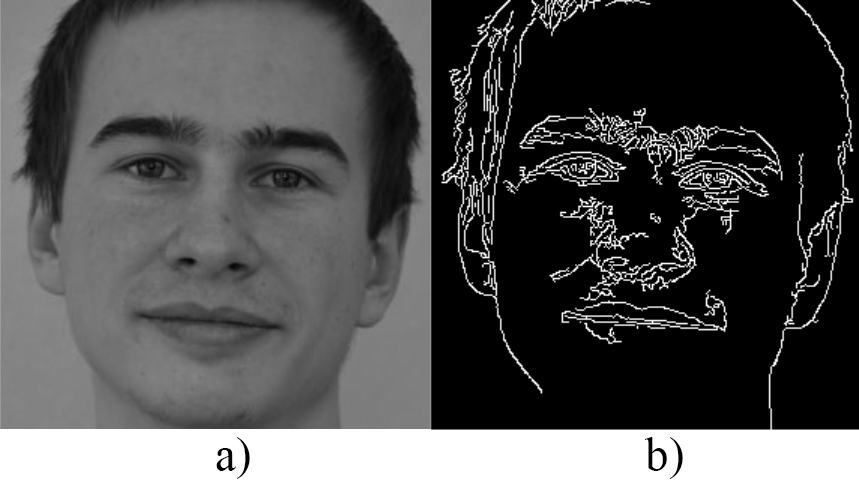
\includegraphics[width=11cm]{Obrazy/mojaTwarzGray.jpg}
        \caption{a) Oryginalny obraz b) Obraz z wykrytymi krawędziami.}
        \label{fig.mojaTwarzGray}
    \end{figure}

    Na Rysunku \ref{fig.mojaTwarzGray} widoczne są krawędzie, które wyróżniają tło od twarzy.
    Ponadto widoczne są poszczególne części twarzy tj. nos, oczy, brwi.
    Można także zauważyć dodatkowe krawędzie w strefach zmarszczkowych (Sekcja \ref{sec:wyznaczanieStref}),
    które identyfikują zmarszczki.
    Ilość białych pikseli w strefach zmarszczkowych jest wprost proporcjonalna do ilości zmarszczek na twarzy danej
    osoby.

    Z każdej strefy zmarszczkowej obliczany jest stosunek ilości białych pikseli do wszystkich
    pikseli(Wzór ~\ref{wzor.wspolczynnikZmarszczek}).
    \large
    \begin{equation}
        W_{s1} = \frac{suma białych pikseli w strefie 1}{suma wszystkich pikseli w strefie 1}
        \label{wzor.wspolczynnikZmarszczek}
    \end{equation}
    \normalsize
    , gdzie $W_{s1}$ jest stosunkiem białych pikseli do wszystkich w strefie 1.
    Analogicznie obliczane są stosunki pikseli dla pozostałych stref.
    Ostatnim etapem jest sumowanie wszystkich stosunków pikseli (Wzór \ref{wzor.wrinkleFeature}).
    \large
    \begin{equation}
        WF = W_{s1} + W_{s2} + W_{s3} + W_{s4} + W_{s5} + W_{s6}
        \label{wzor.wrinkleFeature}
    \end{equation}
    , gdzie WF to wrinkle feature - parametr określający ilość zmarszczek dla danej osoby.
    \normalsize
    \section{Algorytm trenowania}\label{sec:algorytmTrenowania}

    \section{Grupowanie danych - FCM}\label{sec:grupowanieDanych}

    \subsection{Wstęp do grupowania danych}\label{subsec:wstęp-do-grupowania-danych}
    \subsection{Metoda FCM}\label{subsec:metoda-fcm}

    \section{Wyznaczanie wieku}\label{sec:wyznaczanieWieku}


    %Tutaj powinno byc 5000 slow

    \chapter{Modyfikacje metody bazowej}\label{ch:modyfikacje-metody-bazowej}

    \section{Odjęcie wybranej strefy}\label{sec:odjęcie-wybranej-strefy}

    \subsection{Zmiana algorytmu względem metody bazowej}\label{subsec:zmiana-algorytmu-względem-metody-bazowej}

    \section{Zastosowanie metody HOG}\label{sec:zastosowanie-metody-hog}
    \subsection{Opis algorytmu HOG}\label{subsec:opis-algorytmu-hog}
    \subsection{Zastosowanie w projekcie}\label{subsec:zastosowanie-w-projekcie2}

    \section{Metoda HOG oraz grupowanie KNN}\label{sec:metoda-hog-oraz-grupowanie-knn}
    \subsection{Grupowanie KNN}\label{subsec:grupowanie-knn}
    \subsection{Zastosowanie w projekcie}\label{subsec:zastosowanie-w-projekcie}
    %Tutaj powinno byc okolo 7000
    \chapter{Badania}\label{ch:badania}

    %opisywac nie tylko wyniki ale tez posrednio co tam lecialo, statystyki, szybkosc dzialania (sredni czas
    %    przetwarzania), zajetosc pamieci
    \chapter{Podsumowanie}\label{ch:podsumowanie}



    %%%%%%%%%%%%%%%%%%%%%%%%%%%%%%%%%%%%%%%%%%
    \backmatter
    \pagenumbering{Roman}
    \stepcounter{stronyPozaNumeracja}
    \setcounter{page}{\value{stronyPozaNumeracja}}

    \pagestyle{tylkoNumeryStron}

    %%%%%%%%%%% bibliografia %%%%%%%%%%%%
    \bibliographystyle{plplain}
    \bibliography{bibliografia}

    %%%%%%%%%  DODATKI %%%%%%%%%%%%%%%%%%%

    \begin{appendices}


        \chapter*{Dokumentacja techniczna}

        \chapter*{Spis skrótów i symboli}

        \begin{itemize}
            \item[DNA] kwas deoksyrybonukleinowy (ang. \ang{deoxyribonucleic acid})
            \item[MVC] model -- widok -- kontroler (ang. \ang{model--view--controller})
            \item[$N$] liczebność zbioru danych
            \item[$\mu$] stopnień przynależności do zbioru
            \item[$\mathbb{E}$] zbiór krawędzi grafu
            \item[$\mathcal{L}$] transformata Laplace'a
        \end{itemize}




        \chapter*{Zawartość dołączonej płyty}

        Do pracy dołączona jest płyta CD z~następującą zawartością:
        \begin{itemize}
            \item praca w~formacie \texttt{pdf},
            \item źródła programu,
            \item zbiory danych użyte w~eksperymentach.
        \end{itemize}

        \listoffigures
        \listoftables

    \end{appendices}


\end{document}


%% Finis coronat opus.